\documentclass[12pt]{article}
\usepackage{sbc-template}
\usepackage{graphicx,url}
\usepackage[utf8]{inputenc}
\usepackage[brazil]{babel}
\usepackage{booktabs}
\usepackage{amsmath}
\usepackage{float}
\sloppy

\title{Predição de Evasão de Clientes (\textit{Churn}) e Estratégias de Retenção Baseadas em Dados no Setor de Telecomunicações}
\author{Arthur V. F. Rodrigues\inst{1}, Caio M. Soares\inst{1},\\
Mírian N. G. dos Santos\inst{1}, Vinicius A. S. de Alencar\inst{1}}
\address{Instituto de Computação -- Universidade Federal de Alagoas (UFAL)\\
Maceió -- AL -- Brasil}

\begin{document}
\maketitle

\begin{abstract}
This paper analyzes the IBM Telco Customer Churn dataset, with 7,043 customers and 19 original predictors, to support retention decisions. We use data cleaning, feature engineering, statistical comparisons and four classification methods, plus a prevalence baseline. A stratified 60/20/20 split separates training, threshold validation and final testing. Random Forest achieved the highest average precision in five-fold training cross-validation. After probability calibration, its test ROC-AUC was 0.843 and average precision was 0.654. A recall-oriented threshold detected 93.6\% of churn cases, with 41.7\% precision. Selecting the top 20\% of test customers captured 49.2\% of observed churn cases. These retrospective results support a prospective pilot; they do not establish causal effects, future prediction performance or campaign profitability.
\end{abstract}

\begin{resumo}
Este artigo analisa a base IBM Telco Customer Churn, com 7.043 clientes e 19 preditores originais, para apoiar decisões de retenção. O estudo inclui limpeza, criação de atributos, comparações estatísticas e quatro modelos de classificação, além de uma referência por prevalência. Uma divisão estratificada em treino, validação e teste separa as etapas experimentais. A Random Forest obteve a maior precisão média na validação cruzada do treino. Após calibração, alcançou AUC-ROC de 0,843 e precisão média de 0,654 no teste. O corte que prioriza revocação identificou 93,6\% dos churns, com precisão de 41,7\%. Os 20\% de clientes de maior risco concentraram 49,2\% dos churns observados. Os resultados fundamentam um piloto prospectivo, sem demonstrar efeito causal, antecipação em produção ou lucro de campanha.
\end{resumo}

\section{Aplicação}\label{sec:aplicacao}
A perda de assinantes, denominada \textit{churn}, reduz a continuidade da receita de uma operadora de telecomunicações. Uma equipe de retenção com orçamento e capacidade limitados precisa escolher quais clientes procurar e quais ações avaliar. Neste estudo, o problema é identificar características associadas ao cancelamento e avaliar um ranking de risco para apoiar essa priorização.

O objetivo definido pela equipe é entender os fatores contratuais, de serviços e de faturamento ligados à evasão e investigar a identificação antecipada de clientes com maior risco. Para isso, buscamos: testar quatro hipóteses da proposta inicial, comparar modelos e propor ações com indicadores de acompanhamento. A base permite uma avaliação retrospectiva. A confirmação de antecipação e de eficácia comercial exige dados anteriores ao evento e um experimento posterior com clientes ativos.

\section{Base de Dados}\label{sec:base}
Utilizamos o CSV local \texttt{WA\_Fn-UseC\_-Telco-Customer-Churn.csv}, da base pública IBM Telco Customer Churn distribuída no Kaggle \cite{telco}. São 7.043 clientes únicos e 21 colunas originais: um identificador, 19 preditores e o alvo \texttt{Churn}. A auditoria encontrou 1.869 respostas \textit{Yes} (26,54\%) e 5.174 \textit{No} (73,46\%), sem IDs ou registros completos duplicados. A origem amostral não assegura representatividade de uma operadora real.

Os preditores abrangem quatro informações demográficas (\texttt{gender}, \texttt{SeniorCitizen}, \texttt{Partner}, \texttt{Dependents}), nove de serviços (telefonia, linhas adicionais, internet, segurança, backup, proteção, suporte e dois serviços de streaming) e seis de contrato e faturamento (\texttt{tenure}, \texttt{Contract}, \texttt{PaperlessBilling}, \texttt{PaymentMethod}, \texttt{MonthlyCharges}, \texttt{TotalCharges}). Os valores monetários mantêm as unidades da base, sem conversão para reais. O arquivo não traz datas que permitam definir e verificar uma janela futura de previsão.

\subsection{Pré-processamento e Engenharia de Atributos}
Preservamos todas as linhas e o CSV original. Removemos espaços externos e convertemos \texttt{TotalCharges}, originalmente textual, para número. Seus 11 valores em branco correspondem a clientes com \texttt{tenure}=0. Assumimos acumulado zero nesses casos e registramos a ausência original em \texttt{TotalChargesAusente}. Essa regra é uma hipótese de domínio, não uma cobrança medida. Outros nulos numéricos, se presentes, seguem para imputação pela mediana aprendida no treino; categorias ausentes seguem para a moda.

Retiramos \texttt{customerID} dos preditores, tratamos \texttt{SeniorCitizen} como categoria e preservamos \textit{No internet service} e \textit{No phone service} como estados distintos de \textit{No}. Validamos categorias, valores não negativos e coerência entre serviços. Perfis iguais de clientes com IDs diferentes permanecem na base. A inspeção por intervalo interquartil no treino não motivou exclusão automática de valores plausíveis.

Criamos \texttt{ServicosAdicionais}, contagem dos seis serviços de internet com resposta \textit{Yes}, e \texttt{GastoMedioHistorico}, definido por \texttt{TotalCharges}/\texttt{tenure}. A razão fica ausente quando a permanência é zero, evitando divisão inválida, e recebe imputação no pipeline. Com o indicador de ausência, são 22 atributos antes da codificação. Não usamos a razão entre cobrança mensal atual e média histórica descrita como possibilidade em versões preliminares do texto.

O \textit{One-Hot Encoding}, a imputação e o \textit{StandardScaler} ficam em um \texttt{Pipeline}/\texttt{ColumnTransformer}, ajustados dentro de cada dobra de treinamento. Assim, as estatísticas aprendidas não usam validação ou teste. O módulo \texttt{telco\_pipeline.py} contém os tratamentos reutilizáveis, e o notebook registra versões, semente, partições e hash SHA-256 do CSV.

\section{Estatística Descritiva e Inferência}\label{sec:estatistica}
As análises exploratórias e inferenciais usam apenas os 4.225 clientes do treino. A prevalência global apresentada na auditoria descreve a estrutura do arquivo. No treino, há 1.121 churns e 3.104 não churns. A Tabela~\ref{tab:descritiva} mostra as variáveis numéricas após a limpeza determinística. IIQ indica a diferença entre os quartis 75\% e 25\%.

\begin{table}[htbp]
\centering\small
\caption{Estatísticas no treino, por churn. Cobranças em unidades monetárias da base.}
\label{tab:descritiva}
\begin{tabular}{llrrr}\toprule
Variável & Grupo & Média $\pm$ DP & Mediana & IIQ\\\midrule
\texttt{tenure} & Não churn & 37,52 $\pm$ 24,27 & 37,00 & 46,00 \\
\texttt{tenure} & Churn & 17,82 $\pm$ 19,43 & 10,00 & 27,00 \\
\texttt{MonthlyCharges} & Não churn & 61,25 $\pm$ 30,96 & 64,38 & 61,90 \\
\texttt{MonthlyCharges} & Churn & 74,54 $\pm$ 24,62 & 79,75 & 38,45 \\
\texttt{TotalCharges} & Não churn & 2560,79 $\pm$ 2349,61 & 1672,10 & 3734,88 \\
\texttt{TotalCharges} & Churn & 1517,74 $\pm$ 1875,06 & 679,30 & 2146,00 \\
\bottomrule\end{tabular}
\end{table}

Definimos os contrastes das hipóteses: H1 compara contrato mensal com contratos de um/dois anos; H2 compara permanência até 12 meses com mais de 12 meses; H3 compara, somente na fibra, falta de segurança \emph{ou} suporte com presença de ambos; H4 compara cheque eletrônico com débito/cartão automáticos, somente entre faturas a partir de 89,75, o percentil 75 aprendido no treino. H4 exclui cheque pelo correio. H2 não estima risco longitudinal, e H4 não testa formalmente uma interação de preço com pagamento.

Aplicamos testes bilaterais de qui-quadrado de Pearson às quatro tabelas $2\times2$, com correção de Holm dos quatro valores-$p$ e nível de 5\%. As frequências esperadas permitiram o qui-quadrado em todos os contrastes; o código prevê Fisher para tabelas esparsas. Estimamos taxas, intervalos de Wilson, diferença em pontos percentuais e razão de riscos (RR). Os ICs individuais de RR não recebem ajuste por multiplicidade. A significância considera o valor-$p$ corrigido, não esses ICs isoladamente.

\begin{table}[htbp]
\centering\small
\caption{Hipóteses no treino. Taxas: exposto/comparação; RR com IC individual de 95\%.}
\label{tab:hipoteses}
\begin{tabular}{lrrll}\toprule
Hip. & $n_1/n_0$ & Churn (\%) & RR (IC95\%) & $p$ de Holm\\\midrule
H1 & 2326/1899 & 43,1/6,3 & 6,87 (5,74--8,23) & $1,79\times10^{-159}$ \\
H2 & 1318/2907 & 47,3/17,1 & 2,76 (2,50--3,04) & $2,04\times10^{-93}$ \\
H3 & 1636/207 & 45,9/14,0 & 3,28 (2,33--4,61) & $4,24\times10^{-18}$ \\
H4 & 480/521 & 47,1/21,7 & 2,17 (1,80--2,62) & $2,23\times10^{-17}$ \\
\bottomrule\end{tabular}
\end{table}

Os quatro contrastes mostram associação no sentido previsto. As diferenças de taxas são 36,8 pontos percentuais em H1, 30,1 em H2, 31,9 em H3 e 25,4 em H4. Os valores de V de Cramér são, respectivamente, 0,415, 0,316, 0,204 e 0,268. Como complemento exploratório, Mann-Whitney indica distribuições de permanência diferentes entre os grupos ($U=902945{,}5$, $p=1{,}94\times10^{-126}$), com medianas de 10 meses nos churns e 37 nos demais. O efeito rank-biserial é $-0{,}481$. Esse teste não integra a família confirmatória H1--H4 nem equivale, em geral, a testar igualdade de medianas.

\begin{figure}[htbp]
\centering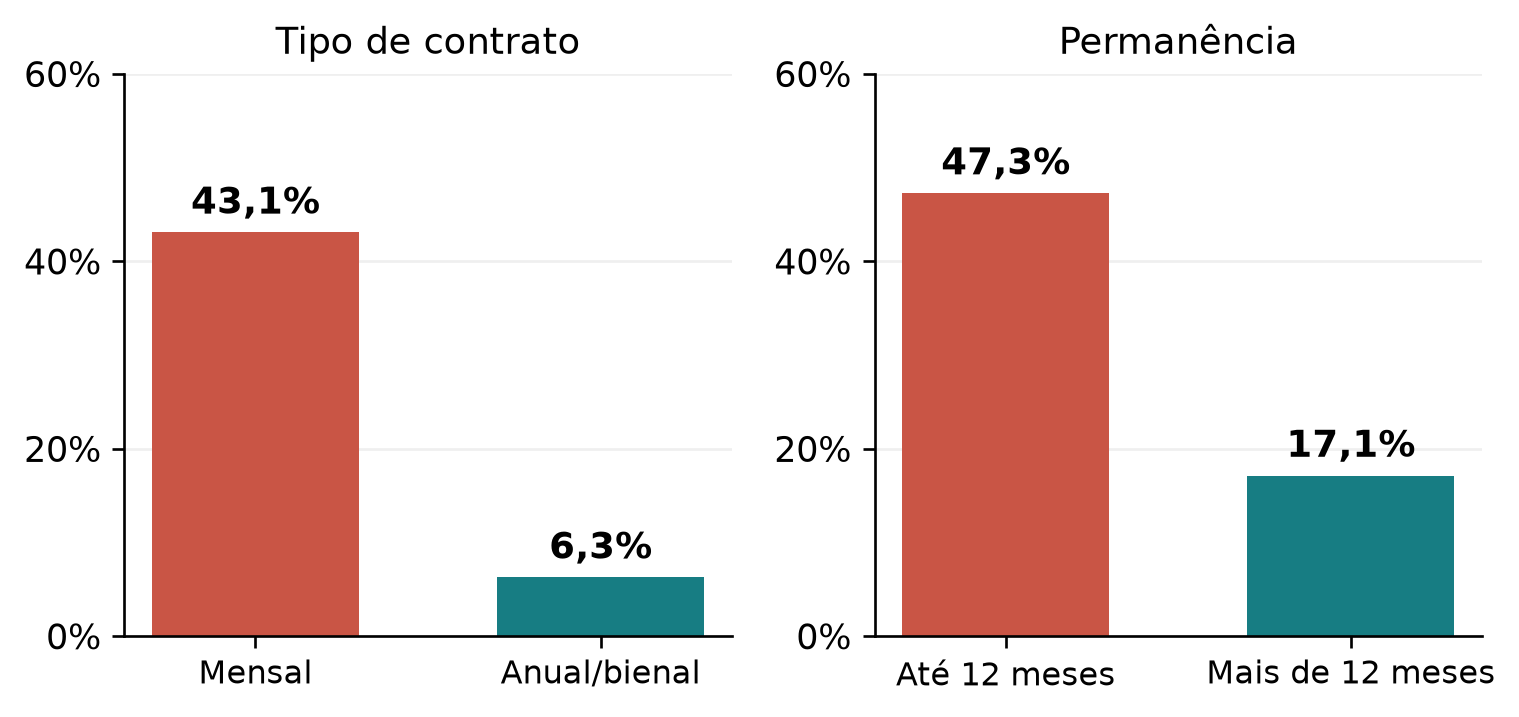
\includegraphics[width=0.95\textwidth]{churn_perfis.png}
\caption{Taxas no treino por contrato e permanência. São associações observacionais, sem ajuste por outros fatores.}
\label{fig:perfis}
\end{figure}

Na correlação de Spearman do treino, permanência e cobrança acumulada têm correlação de aproximadamente 0,90. Cobrança mensal e gasto médio histórico têm correlação próxima de 0,99, mostrando redundância entre atributos financeiros. Esses padrões ajudam a descrever a amostra, mas não demonstram que alterar contrato, suporte ou pagamento reduzirá o cancelamento. H2 também pode refletir viés de sobrevivência: clientes que permanecem acumulam mais meses de relacionamento.

\section{Métodos Avaliados}\label{sec:metodos}
Implementamos os métodos no scikit-learn \cite{pedregosa2011}. A Regressão Logística é uma referência regularizada de interpretação mais simples. A Árvore de Decisão captura regras e interações não lineares, com profundidade controlada. A \textit{Random Forest} combina árvores para reduzir a variância, embora ainda possa sobreajustar. O \textit{HistGradientBoosting} representa o boosting com regularização. Optamos pela implementação nativa em vez das dependências adicionais XGBoost/LightGBM, citadas inicialmente como possibilidades. Um \texttt{DummyClassifier(strategy='prior')} fornece a referência sem informações dos atributos.

A busca em grade avalia: na Logística, $C\in\{0{,}1;1\}$ e pesos ausentes ou balanceados; na Árvore, profundidade 3 ou 6, folha mínima 25 e pesos ausentes ou balanceados; na Forest, 180 árvores, profundidade 8 ou ilimitada, folha mínima 5 e pesos ausentes ou \texttt{balanced\_subsample}; no boosting, 160 iterações, 7 ou 15 folhas máximas, regularização L2 igual a 1 e pesos ausentes ou balanceados. Não aplicamos SMOTE antes da divisão.

\section{Métricas de Avaliação}\label{sec:metricas}
A métrica primária de seleção é \textit{average precision} (AP), resumo da curva precisão-revocação calculado pela implementação oficial \cite{ap}. AP não é a área trapezoidal sob essa curva e não representa porcentagem de acertos. A referência por prevalência permite interpretar o ganho sobre uma lista sem informação. AUC-ROC avalia ordenação de risco, também sem corresponder a acurácia.

Precisão e revocação, para verdadeiros positivos VP, falsos positivos FP e falsos negativos FN, são $P=VP/(VP+FP)$ e $R=VP/(VP+FN)$. F1 equilibra as duas. Para escolher o corte, usamos $F_2=5PR/(4P+R)$, que dá maior peso à revocação. Essa preferência é uma decisão didática de priorização de detecção, não uma otimização de lucro. Acurácia, acurácia balanceada, matriz de confusão e Brier complementam a avaliação; Brier mede erro quadrático das probabilidades, com valores menores preferíveis.

\section{Métodos de Avaliação}\label{sec:avaliacao}
Com semente 42, reservamos inicialmente 20\% para teste e dividimos os demais em treino e validação. O resultado é 4.225 clientes no treino (aproximadamente 60\%), 1.409 na validação (20\%) e 1.409 no teste (20\%), com estratificação e sem interseção de IDs. Não há datas para uma validação temporal.

A seleção de modelo e hiperparâmetros usa AP média em \textit{Stratified K-Fold} de cinco dobras no treino. As médias de seleção podem ser otimistas após a busca; seus desvios entre dobras não são ICs. Após selecionar o método, aplicamos calibração sigmoid com três dobras estratificadas, também somente no treino \cite{calibracao}. O ensemble calibrado mantém três pipelines, cada qual com transformações ajustadas em seu subconjunto de treinamento.

A validação separada escolhe o corte que maximiza F2, com desempate pelo maior corte, resultando em 0,10035. Mantemos o modelo ajustado apenas no treino: retreinar com validação alteraria a escala usada para escolher o corte. O teste final avalia somente a solução congelada e a referência Dummy. Não escolhemos novamente modelo, atributos ou corte após consultar esse conjunto.

Calculamos ICs percentis por 500 reamostragens bootstrap estratificadas dos pares rótulo/previsão do teste, sem retreinar. Esses ICs são condicionais ao modelo e à proporção de classes observada; não incluem incerteza de seleção ou mudanças futuras da população. A interpretação por permutação usa a validação, preservando o teste para a avaliação final.

\section{Resultados e Discussão}\label{sec:resultados}
A Tabela~\ref{tab:modelos} compara as melhores configurações de cada método em validação cruzada. A Forest obteve AP de 0,672, próxima da Logística (0,667) e do boosting (0,662). A diferença é pequena e não fizemos teste de superioridade estatística entre modelos. A configuração selecionada tem profundidade 8 e não usa pesos de classe. Sua AP no próprio treino é 0,789, maior que a média de CV; não interpretamos esse resultado aparente como desempenho fora da amostra.

\begin{table}[htbp]
\centering\small
\caption{Seleção no treino: média de CV. DP é a dispersão entre dobras; F1 usa corte 0,5.}
\label{tab:modelos}
\begin{tabular}{lrrr}\toprule
Modelo & AP $\pm$ DP & AUC-ROC & F1\\\midrule
\textit{Random Forest} & 0,672 $\pm$ 0,011 & 0,848 & 0,572 \\
Regressão Logística & 0,667 $\pm$ 0,025 & 0,848 & 0,598 \\
\textit{HistGradientBoosting} & 0,662 $\pm$ 0,016 & 0,842 & 0,582 \\
Árvore de Decisão & 0,603 $\pm$ 0,021 & 0,817 & 0,551 \\
Referência por prevalência & 0,265 $\pm$ 0,000 & 0,500 & 0,000 \\
\bottomrule\end{tabular}
\end{table}

Após calibração, a Forest alcança AUC-ROC de 0,843 no teste (IC95\% bootstrap: 0,823--0,864) e AP de 0,654 (0,613--0,698). Seu Brier é 0,137, comparado a 0,195 da referência. A Tabela~\ref{tab:teste} mostra o efeito de mudar o corte da mesma solução congelada. O corte 0,5 é apenas referência operacional, não uma nova seleção no teste.

\begin{table}[htbp]
\centering\small
\caption{Teste final. Acurácia, precisão e revocação em porcentagem. RF: Forest calibrada.}
\label{tab:teste}
\begin{tabular}{lrrrrr}\toprule
Solução (corte) & Acur. & Precisão & Revocação & F1 & F2\\\midrule
Referência (0,5) & 73,5 & 0,0 & 0,0 & 0,000 & 0,000 \\
RF calibrada (0,5) & 79,4 & 64,8 & 49,2 & 0,559 & 0,517 \\
RF calibrada (F2) & 63,6 & 41,7 & 93,6 & 0,577 & 0,749 \\
\bottomrule\end{tabular}
\end{table}

No corte F2, o modelo identifica 350 dos 374 churns do teste e deixa passar 24. Entretanto, sinaliza 839 clientes (59,5\%), dos quais 489 não cancelaram; 546 não churns ficam sem sinalização. A revocação de 93,6\% exige, portanto, muitos contatos e tem precisão de 41,7\%. Sua acurácia de 63,6\% é inferior aos 73,5\% da referência que sempre prevê não churn. Isso não invalida a detecção, mas evidencia o custo de priorizar revocação. Os ICs condicionais são 90,9--96,1\% para revocação e 40,0--43,5\% para precisão.

Uma alternativa com capacidade limitada é selecionar o topo do ranking. As frações de 10\%, 20\%, 30\% e 50\% foram definidas como cenários, sem otimização no teste. Usamos arredondamento para cima na quantidade de contatos. Como mostra a Tabela~\ref{tab:capacidade}, os 20\% de maior risco correspondem a 282 clientes e incluem 184 churns: captura de 49,2\%, precisão de 65,2\% e lift de 2,46 em relação à prevalência. Seleção aleatória de 20\% alcançaria 20\% dos churns em expectativa. Não realizamos uma campanha aleatória de comparação.

\begin{table}[htbp]
\centering\small
\caption{Capacidade de contato no teste retrospectivo. Captura: fração dos 374 churns alcançados.}
\label{tab:capacidade}
\begin{tabular}{rrrrrr}\toprule
Capacidade & Contatos & Churns & Precisão & Captura & Lift\\\midrule
10\% & 141 & 109 & 77,3\% & 29,1\% & 2,91 \\
20\% & 282 & 184 & 65,2\% & 49,2\% & 2,46 \\
30\% & 423 & 248 & 58,6\% & 66,3\% & 2,21 \\
50\% & 705 & 324 & 46,0\% & 86,6\% & 1,73 \\
\bottomrule\end{tabular}
\end{table}

\begin{figure}[htbp]
\centering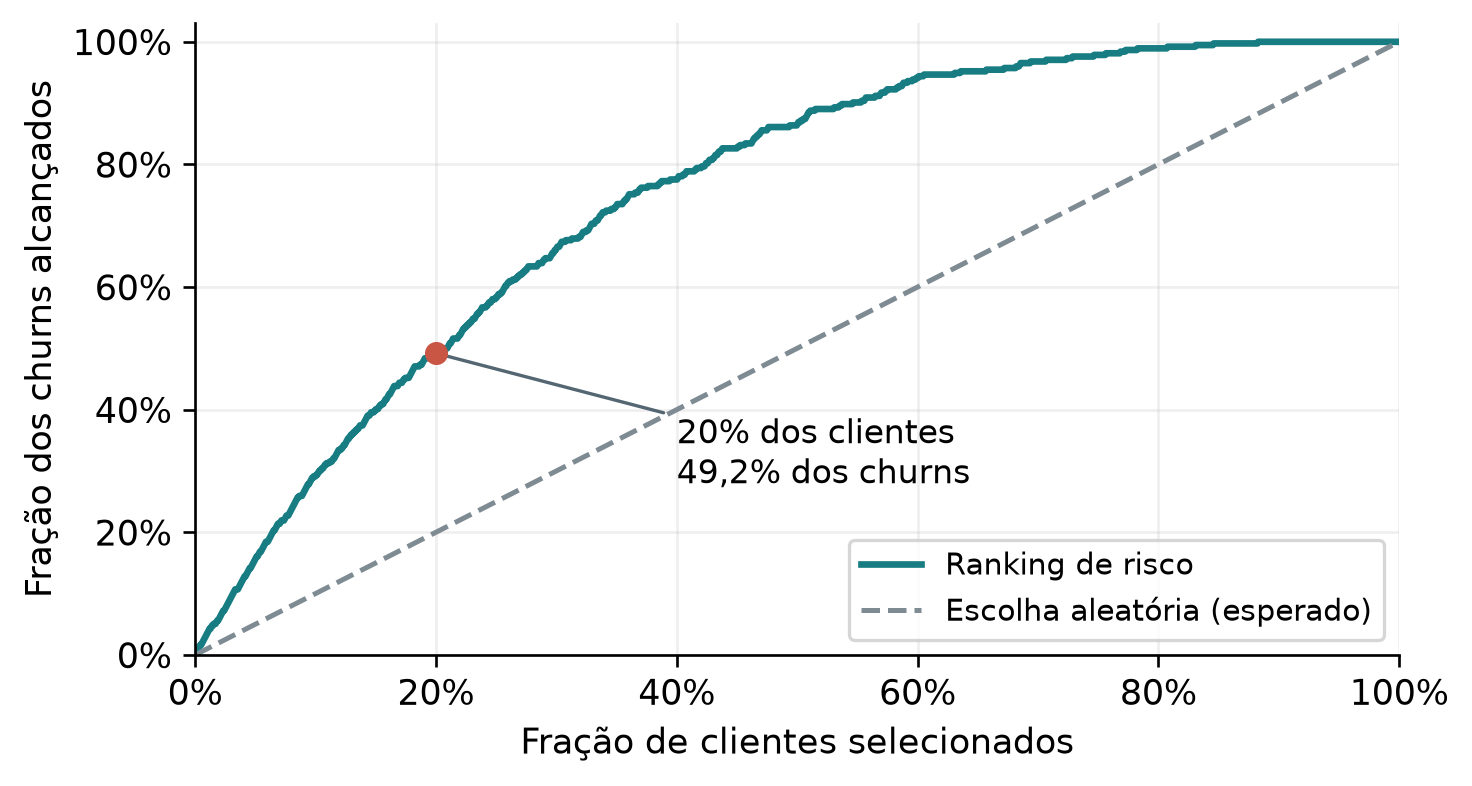
\includegraphics[width=0.88\textwidth]{churn_captura.png}
\caption{Captura cumulativa no ranking do teste. Alcançar churns observados não implica evitá-los.}
\label{fig:captura}
\end{figure}

Para interpretar o ranking, permutamos colunas na validação e medimos a queda de AP em oito repetições. Internet e seus seis serviços foram permutados em bloco, assim como telefonia e múltiplas linhas, evitando combinações de cadastro impossíveis. As maiores quedas médias ocorreram em internet/serviços (0,127), permanência (0,069) e contrato (0,066). Cobrança acumulada teve queda de 0,009. A importância de um bloco depende de sua composição e não é comparável a um efeito individual causal; atributos correlacionados podem repartir importância.

\subsection{Insights Acionáveis e Recomendações de Negócio}
Os resultados apoiam quatro propostas, condicionadas a validar a disponibilidade dos atributos antes da saída e a estabelecer uma capacidade de contato. Um piloto prospectivo de 90 dias deve sortear tratamento e controle dentro de cada perfil, medir churn e margem incremental e registrar custo de oferta. A meta sugerida, ainda não observada, é reduzir o churn em pelo menos 10\% em termos relativos, com IC da diferença abaixo de zero e margem incremental positiva. O tamanho da amostra e os ajustes por múltiplas ações precisam de planejamento anterior ao piloto.

\begin{itemize}
\item \textbf{Contrato:} a taxa de 43,1\% no mensal, contra 6,3\% nos contratos mais longos, justifica testar migração voluntária para um plano anual. O valor do benefício depende da margem disponível. Acompanhar churn e margem por cliente contatado, comparados ao controle.
\item \textbf{Permanência:} a taxa de 47,3\% até 12 meses, contra 17,1\% acima disso, motiva testar acompanhamento nos primeiros meses. Acompanhar churn, satisfação e custo por cliente retido.
\item \textbf{Fibra e suporte:} as taxas de 45,9\% e 14,0\% motivam diagnóstico técnico e oferta de segurança/suporte para o perfil correspondente. Acompanhar churn, resolução de chamados e margem. A análise não estima o efeito de conceder suporte gratuito.
\item \textbf{Cobrança e pagamento:} entre faturas altas, as taxas de 47,1\% no cheque eletrônico e 21,7\% no automático justificam testar esclarecimento de cobrança e adesão voluntária ao pagamento recorrente. Acompanhar churn, adesão e margem.
\end{itemize}

\subsection{Simulação Financeira}
Para ilustrar a ligação com a decisão, fixamos contato com os 20\% de maior risco, custo de 10 unidades por contato, horizonte de três meses e margem de contribuição de 40\% sobre a cobrança. A eficácia de retenção é hipotética: 10\%, 20\% ou 30\% dos churns alcançados seriam evitados. Usamos os rótulos retrospectivos para calcular o benefício simulado, sem estimar essa eficácia pelo modelo:
\[
 B=e\sum_{i\in S,\,y_i=1}3\,(0{,}40)\,\texttt{MonthlyCharges}_i,
 \qquad L=B-10|S|.
\]
Aqui, $S$ é o grupo de 282 contatos, $e$ é a eficácia assumida, $B$ o benefício e $L$ o saldo simulado. O custo total é 2.820 unidades. A eficácia de equilíbrio é aproximadamente 16,5\%. Esses valores não são reais brasileiros nem resultados de uma ação executada.

\begin{table}[htbp]
\centering\small
\caption{Cenários hipotéticos, em unidades monetárias da base.}
\label{tab:financeiro}
\begin{tabular}{rrrr}\toprule
Eficácia & Custo & Benefício simulado & Saldo simulado\\\midrule
10\% & 2820,00 & 1709,15 & -1110,85 \\
20\% & 2820,00 & 3418,31 & 598,31 \\
30\% & 2820,00 & 5127,46 & 2307,46 \\
\bottomrule\end{tabular}
\end{table}

A simulação não inclui desconto nas ofertas, custos adicionais, valor do dinheiro no tempo ou resposta diferenciada dos clientes. Portanto, não estima CLV nem demonstra lucro. Um modelo de risco não identifica necessariamente quem responderá melhor à intervenção; essa pergunta exige efeito de tratamento ou \textit{uplift}, ausentes neste estudo.

\subsection{Limitações do Estudo}
A base é observacional e amostral, sem datas suficientes para uma avaliação temporal. Atributos de permanência e cobrança podem refletir o próprio processo de saída. Precisamos confirmar sua disponibilidade antes do evento e definir uma janela futura, sem a qual não demonstramos antecipação em produção. As associações podem sofrer influência de fatores não medidos e de viés de sobrevivência.

A validação orientou o corte e a interpretação; suas métricas são de desenvolvimento. O teste é independente desse ajuste, mas os ICs não incluem a incerteza de todo o treinamento e seleção. A busca de hiperparâmetros foi limitada, e não fizemos ablação para atribuir ganho às variáveis derivadas. Sexo/gênero e idade constam entre os preditores; seu uso real exige avaliar necessidade, disparidades entre grupos e critérios de atendimento. Não realizamos auditoria completa de equidade. O dashboard Streamlit da proposta permanece como extensão, sem implementação nesta entrega.

\section{Conclusão}\label{sec:conclusao}
O estudo reuniu auditoria, preparação, inferência e classificação para apoiar a priorização de retenção. Encontramos associação entre churn e contratos mensais, permanência curta, falta de segurança/suporte na fibra e cheque eletrônico entre faturas altas. A Forest teve a maior AP na CV, com pequena diferença para a Logística. Após calibração, alcançou AUC-ROC de 0,843 e AP de 0,654 no teste.

O corte F2 identifica 93,6\% dos churns com muitos alertas: precisão de 41,7\% e 59,5\% dos clientes sinalizados. Para uma capacidade de 20\%, o ranking concentra 49,2\% dos churns, com precisão de 65,2\%. Esses resultados ajudam a escolher quem procurar primeiro. A confirmação de antecipação, redução de cancelamentos e retorno financeiro depende de avaliação temporal e piloto com clientes ativos e controle aleatório. O artigo propõe esse próximo passo, sem declarar efeitos de campanha que não foram medidos.

\begin{thebibliography}{9}
\bibitem{telco} BlastChar. \textbf{Telco Customer Churn}. Kaggle Datasets. Disponível em: \url{https://www.kaggle.com/datasets/blastchar/telco-customer-churn}. Base local consultada em 15 nov. 2026.
\bibitem{pedregosa2011} Pedregosa, F. et al. \textbf{Scikit-learn: Machine Learning in Python}. Journal of Machine Learning Research, v. 12, p. 2825--2830, 2011. \url{https://jmlr.org/papers/v12/pedregosa11a.html}.
\bibitem{ap} Scikit-learn Developers. \textbf{average\_precision\_score}. Documentação da versão 1.9.1. \url{https://scikit-learn.org/stable/modules/generated/sklearn.metrics.average_precision_score.html}. Acesso em: 15 nov. 2026.
\bibitem{calibracao} Scikit-learn Developers. \textbf{Probability calibration}. Documentação da versão 1.9.1. \url{https://scikit-learn.org/stable/modules/calibration.html}. Acesso em: 15 nov. 2026.
\end{thebibliography}
\end{document}
